\documentclass[a4paper,11pt]{article}
\usepackage[italian]{babel}
\usepackage[T1]{fontenc}
\usepackage[utf8]{inputenc}
\usepackage{amsmath}
\usepackage{amsthm}
\usepackage[a4paper,top=1.5cm,bottom=2cm,left=1.5cm,right=1.5cm]{geometry}
\usepackage{amsfonts}
\usepackage{color}
\usepackage{bbm}
\usepackage{datetime}
\usepackage[colorlinks=true]{hyperref}
\usepackage{graphicx}
\usepackage{verbatim}
\usepackage{titlepic}
%\usepackage{physics}
\usepackage{subfigure}
\usepackage{float}

\newcommand{\abs}[1]{\lvert#1\rvert}

\begin{document}

\title{\sc Homework 2}
\author{\sc Alice Schirinà}
\maketitle

\noindent Consideriamo un sistema di molecole monoatomiche che interagiscono tramite un potenziale accoppiato così definito:
\begin{equation*}
V(r) = A \left( \frac{\sigma}{r}\right)^{12} - B \left( \frac{\sigma}{r}\right)^6
\end{equation*}
quando $ r <r_c $, dove $ r_c $ è detto raggio di $\textit{cut-off}$, e $V(r) =0$ per $ r >r_c $. Fissiamo $ A/B =1$, $\rho \sigma^3=0.5$ e utilizziamo unità ridotte, ovvero in ogni simulazione calcoliamo $ E^*=E/k_BT$ e $ P^*=P\sigma^3/k_BT $. \\
Inizialmente le molecole sono uniformemente distribuite in maniera casuale in una scatola cubica di lato $ L/\sigma $. Spostiamo poi le molecole sequenzialmente utilizzando l'algoritmo di Metropolis, proponendo quindi lo spostamento
\begin{eqnarray*}
	x'&=&x+\Delta (r_1 - 0.5)\\
	y'&=&y+\Delta (r_2 - 0.5)\\
	z'&=&z+\Delta (r_3 - 0.5)\\
\end{eqnarray*}
\medskip
dove gli $ r_i $ con $ i=1,2,3$ sono numeri distribuiti uniformemente in $[0,1]$.

\section*{Role of $\Delta$}
\noindent Consideriamo un sistema di $N$ molecole confinate in una scatola cubica di lato $L/\sigma$ fissato in maniera tale che sia $\rho \sigma^3 = 0.5$. Eseguiamo una simulazione che consiste di $5000$ passi Montecarlo per ogni valore di $\Delta$ e stabiliamo quale sia il suo range ottimale, cioè quei valori che minimizzano l'errore.\\ 
Dalle simulazioni osserviamo che l'energia si stabilizza generalmente dopo circa $90$ iterazioni, per questo motivo scartiamo le prime $100$, potendo così osservare valori all'equilibrio per energia e pressione.\\ 
Le correzioni di coda (in unità ridotte) sono:
\begin{eqnarray*}
	\Delta V_t&=&\pi \left(\frac{N}{L^3}\right) \left(\frac{1-3r_c^6}{9r_c^9}\right)\\
	\Delta P_t&=&-2 \pi \left( \frac{N}{L^3} \right)^2 \left(\frac{3r_c^6-2}{9r_c^9}\right)\\
\end{eqnarray*}
\medskip
Per $r_c=L/2$ otteniamo i valori riportati in tabella, dove $N$ è il numero di molecole, $\tau$ il tempo di autocorrelazione e $\sigma$ l'errore sulle stime di energia e pressione. \\
\medskip 
\begin{table}[H]
	\centering
	\begin{tabular}{cccccccccc} 
		\hline
		$\Delta$	&	$ \langle A \rangle $	&	$ \langle E \rangle $	&	$\Delta E_T$	&	$\tau_E$	&	$\sigma_E$	&	$ \langle P \rangle $	&	$\Delta P_T$	&	$\tau_P$	&	$\sigma_P$\\
		\hline
		$1/8$	&	$0.89$	&	$-0.1748$	&	$-0.0348$	&	$13.446$	&	$0.0046$	&	$1.0225$	&	$-0.0349$	&	$20.056$	&	$0.0143$\\
		$1/4$	&	$0.78$	&	$-0.1818$	&	$-0.0348$	&   $3.246$		&	$0.0021$	&	$0.9984$	&	$-0.0349$	&	$4.755$		&	$0.0067$\\
		$1/2$	&	$0.61$	&	$-0.1789$	&	$-0.0348$	&	$2.335$		&	$0.0018$	&	$1.0092$	&	$-0.0349$	&	$3.005$		&	$0.0051$\\
		$1$		&	$0.37$	&	$-0.1768$	&	$-0.0348$	&	$2.099$		&	$0.0017$	&	$1.0154$	&	$-0.0349$	&	$2.156$		&	$0.0045$\\
		$2$		&	$0.18$	&	$-0.1786$	&	$-0.0348$	&	$3.645$		&	$0.0023$	&	$1.0103$	&	$-0.0349$	&	$3.533$		&	$0.0059$\\
		$L/2$	&	$0.14$	&	$-0.1746$	&	$-0.0348$	&	$4.408$		&	$0.0025$	&	$1.0210$	&	$-0.0349$	&	$4.365$		&	$0.0065$\\
		\hline
	\end{tabular}
\end{table}
\medskip
\noindent Da questi possiamo dedurre che i valori ottimali di $\Delta$ sono $1/2$ e $1$. Ricordiamo che i valori sono espressi in unità di $\sigma$ e che i valori di $ \langle P \rangle $ contengono già il contributo ideale $P^*_{id}= 0.5$.\\

\section*{Role of the cute-off}
\noindent Prendiamo nuovamente un sistema con $N=60$ molecole. Fissiamo ora $\Delta=1$ ed eseguiamo due simulazioni con differenti valori di $r_c$.
\begin{table}[H]
	\centering
	\begin{tabular}{ccccc} 
		\hline
		$r_c$ & $\langle E \rangle $ & $\Delta E_T$ & $ \langle P \rangle $ & $\Delta P_T$\\
		\hline
		$3L/8$	&	$-0.1294$	&	$-0.0821$	&	$1.0618$	&	$-0.0814$	\\
		$L/4$	&	$0.0439$	&	$-0.2528$	&	$1.2232$	&	$-0.2263$	\\\hline
	\end{tabular}
\end{table}
\medskip
\noindent Come ci aspettavamo la correzione di coda diventa sempre più rilevante man mano che $r_c$ diminuisce. 

\section*{Size effects}
\noindent Infine consideriamo due sistemi con numero di molecole diverso ed eseguiamo le simulazioni fissando $r_c=L/2$ e nuovamente $\Delta =1$.
\begin{table}[H]
	\centering
	\begin{tabular}{ccccc} 
		\hline
		$N$ & $\langle E \rangle $ & $\Delta E_T$ & $ \langle P \rangle $ & $\Delta P_T$\\
		\hline
		$100$	&	$-0.1901$	&	$-0.0210$	&	$1.0048$	&	$-0.0208$\\
		$200$	&	$-0.1961$	&	$-0.0105$	&	$0.9941$	&	$-0.0105$\\
		\hline
	\end{tabular}
\end{table}
\medskip
\noindent In particolare consideriamo il sistema con $N=200$ molecole e calcoliamo la funzione di distribuzione accoppiata come segue:
\begin{equation*}
	g^{(2)}(R) =V \langle \delta (R-r_{ij}) \rangle
\end{equation*}
\medskip
da cui otteniamo per $R=n \epsilon$ l'espressione
\begin{equation*}
g^{(2)}(n \epsilon) = \frac{2V}{N(N-1) V_s(n, \epsilon)} h(n)
\end{equation*}
\medskip
dove $\epsilon$ è un numero sufficientemente piccolo che rappresenta lo spessore di un guscio sferico $V_s$. La funzione $h(n)$ conta le coppie di particelle tali che $R<r_{ij}<R+\epsilon$. \\
Fissiamo, quindi, $\epsilon = 1/20$ (unità ridotte) e calcoliamo e mediamo la $g^{(2)}(n \epsilon)$ sulle iterazioni all'equilibrio.
\begin{figure}[H]
	\centering 
	%\subfigure[]
	{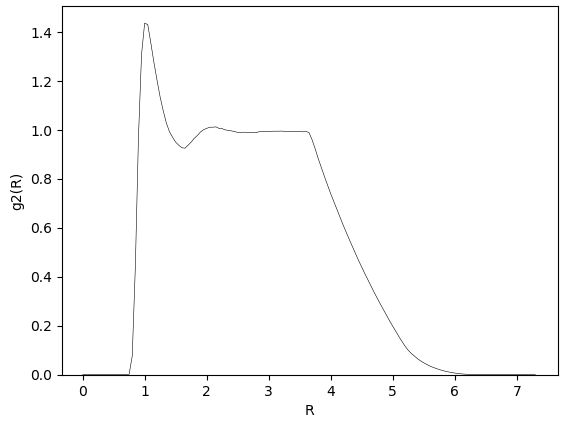
\includegraphics[width=0.8\linewidth]{graficoG2}}
\end{figure}
\medskip

\section*{Physical units}
\noindent Siano ora $A/k_B=150 K$ e $\sigma=0.30 nm$. Utilizziamo i valori trovati nella simulazione con $N=200$ della precedente sezione e calcoliamo la densità molare, l'energia per particella e la pressione:
\begin{eqnarray*}
	\rho_{mol} &=& \frac{1}{2 \sigma^3 N_A} =3.75 \times 10^{-2}\quad mol/cm^3 \\	
	E &=& \frac{E^*}{kT} = -4.8 \times 10^{-3}\quad eV\\
	P &=& P^* \frac{kT}{\sigma^3} = 1.52 \times 10^{8}\quad Pa\\
\end{eqnarray*}
\medskip



\end{document}